\chapter{The Interactive Application}
\label{chap_app}

This chapter presents the interactive application built on top of the RAG pipeline, which is the primary user-facing deliverable of the thesis. It first describes the web interface and how a user configures and converses with the system, then introduces the two conversational memory strategies the application offers, and finally uses the application to compare those two strategies in a multi-turn setting that the automated evaluation of Chapter~\ref{chap6} could not distinguish. The complete source code for the application is available at \url{https://github.com/adrewkan/Thesis}.

\section{Web Interface}

The primary deliverable of the thesis is an interactive web application that exposes the full RAG pipeline through a browser-based chat interface, built with Streamlit \cite{streamlit2019} and run locally. It lets a user hold a natural-language conversation about the loaded contracts without any programming knowledge, and switch between every experimental axis of the thesis from a single configuration panel.

The web app UI is visible in Figure ~\ref{fig:app} below. A sidebar holds the configuration controls. The user selects the language model (Llama~3.1~8B or Mistral~7B), the chunking strategy (fixed, recursive, or semantic, which determines the vector database that is queried), the memory strategy (windowed, with an adjustable window size $k$, or summary), and the number of chunks $k$ to retrieve per query. A ``Load Chain" button assembles the selected configuration, and a ``Clear Chat" button resets the conversation and its memory. A status panel reports the configuration currently loaded. Because loading a quantized language model is the most expensive step, the models and vector stores are cached: switching the chunking strategy or the memory type reuses the already-loaded model rather than triggering a full reload, so only the first load of each model incurs the download and initialization cost.

\begin{figure}[h!]
    \centering
    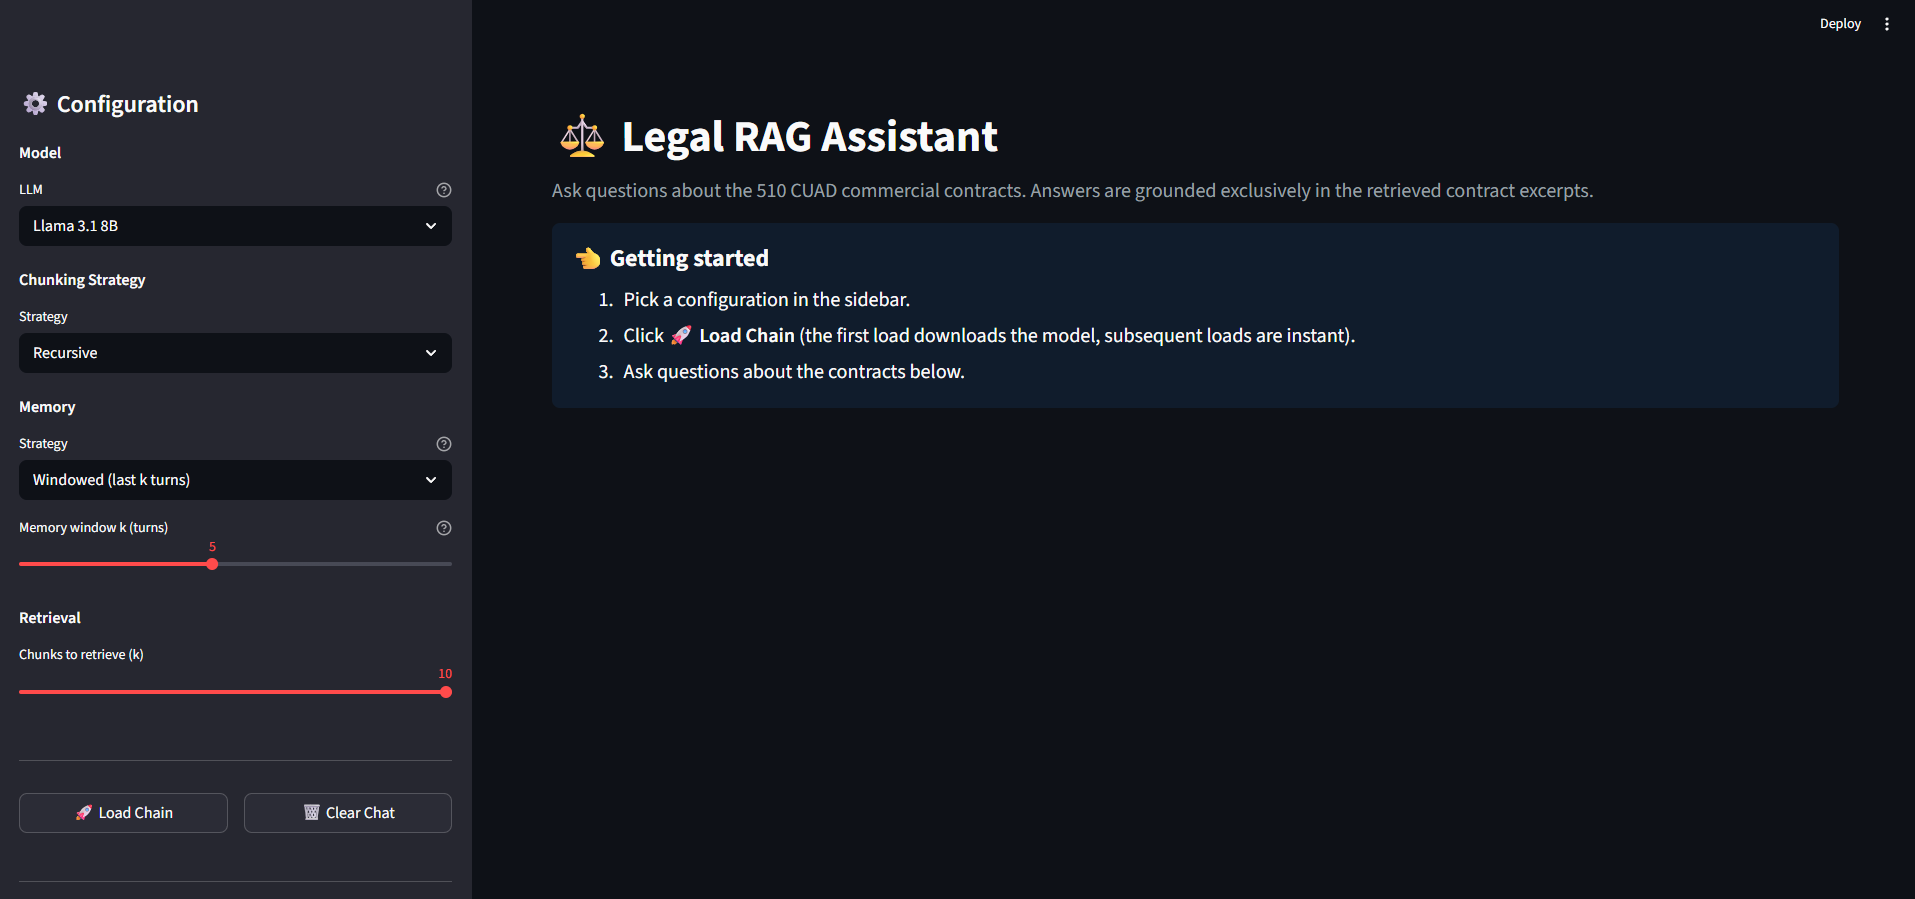
\includegraphics[width=\linewidth]{figures/app.png}
    \caption{The UI of the web application.}
    \label{fig:app}
\end{figure}

The main area is the chat itself. Each user question is answered by the pipeline, and the answer is grounded exclusively in the retrieved contract excerpts. Two details of the pipeline are surfaced in the interface to make its behaviour transparent. First, when conversational memory rewrites a follow-up question into a standalone retrieval query, that reformulated query is shown above the answer, so the effect of the question-condensation step is visible. Second, each answer carries an expandable source-documents panel that lists the retrieved chunks with their source filenames, allowing the user to trace the answer back to the specific contract passages it was drawn from. Both appear in the multi-turn session screenshots shown later in this chapter.

\section{Conversational Memory}

Standard RAG treats each query independently. In a multi-turn conversation, follow-up questions frequently refer to earlier turns. For example, asking ``what does that clause say about liability?" requires knowing which clause was discussed before. Without memory, the system cannot resolve such references. The application implements two approaches, selectable from the sidebar.

\subsection{Windowed Memory}

Windowed memory retains the last $k$ question-answer pairs verbatim and prepends them to the current query before retrieval. Nothing in the retained window is summarized or reinterpreted, so the context passed to the model is exact. In the application these pairs are formatted as alternating Human and Assistant lines, and the window size $k$ is configurable from the sidebar (default $k=5$). The cost is that the prompt grows with each turn: for a window of $k$ pairs, roughly $k$ times the average exchange length is added to every request. In short conversations this is not a problem, but in longer sessions the history eventually competes with the retrieved passages for the model's context window.

\subsection{Summary Memory}

Summary memory replaces the full conversation history with a compressed version generated by the language model. After each exchange, the model updates a running summary using a dedicated prompt that instructs it to preserve key legal details such as clause names, party names, dates, and obligations. Only this summary, rather than the raw history, is included in subsequent prompts. This scales to longer conversations without growing the prompt unboundedly, but the compression is lossy: details that seem unimportant at the time of summarization may become relevant in a later turn, and the summary quality depends on the language model that produces it. The summary-update prompt is shown in Figure~\ref{fig:summary_prompt}.

\begin{figure}[h!]
    \centering
    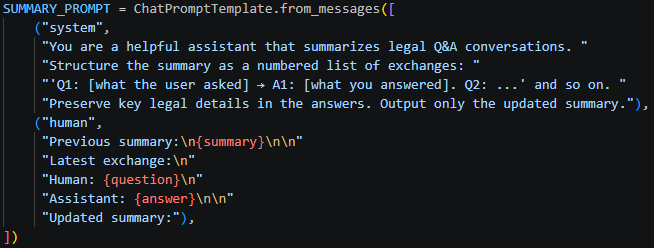
\includegraphics[width=0.87\linewidth]{figures/summary_prompt.png}
    \caption{Summary-memory prompt.}
    \label{fig:summary_prompt}
\end{figure}


\section{Memory Strategy Comparison}
The automated evaluation runs each question in isolation, resetting conversation history before each turn. Both windowed and summary memory are therefore equivalent in that setting. To compare the two strategies in a realistic multi-turn scenario, a fixed sequence of seven questions was run manually through the Streamlit interface, using Llama 3.1 8B as the generator for both the answers and the running summary. The sequence used six questions drawn from the CUAD annotations for a randomly chosen contract (the Sphere 3D Corp consulting agreement), plus one question that references information from a turn before the memory window.

\subsection{Question Sequence}

The six content questions covered the following CUAD categories: (1) contracting parties, (2) effective date, (3) expiration date of the initial term, (4) governing law, (5) consequences of failing to notify before the term ends, and (6) non-compete restrictions. The seventh question was a meta-question asking the model to recall the first question of the session and the answer it gave, without referencing the contract by name.

Question 6 has \texttt{is\_impossible=True} in the CUAD annotations: the Sphere 3D Corp consulting agreement does not contain a non-compete clause. This question was included to verify that the model correctly declines to answer rather than fabricating a clause.

\subsection{Windowed Memory Results}

Questions 1 through 6 were answered correctly under windowed memory ($k=5$). The retrieval query at each turn included the full contract filename, which the condense step reconstructed from conversation history, so retrieval remained contract-specific throughout the session (Figures~\ref{fig:memory1} and~\ref{fig:memory2}).

\begin{figure}[h!]
    \centering
    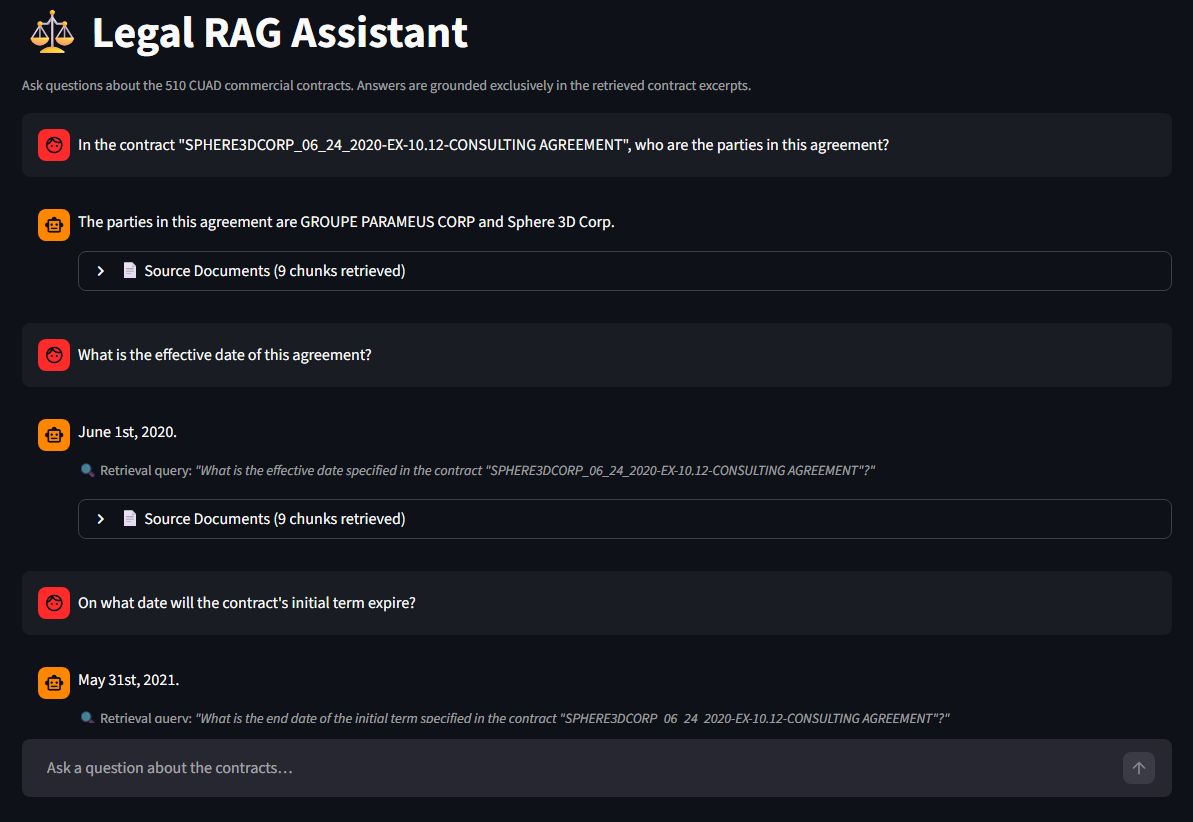
\includegraphics[width=\textwidth]{figures/memory1.png}
    \caption{Windowed memory session, questions 1 to 3.}
    \label{fig:memory1}
\end{figure}

\begin{figure}[h!]
    \centering
    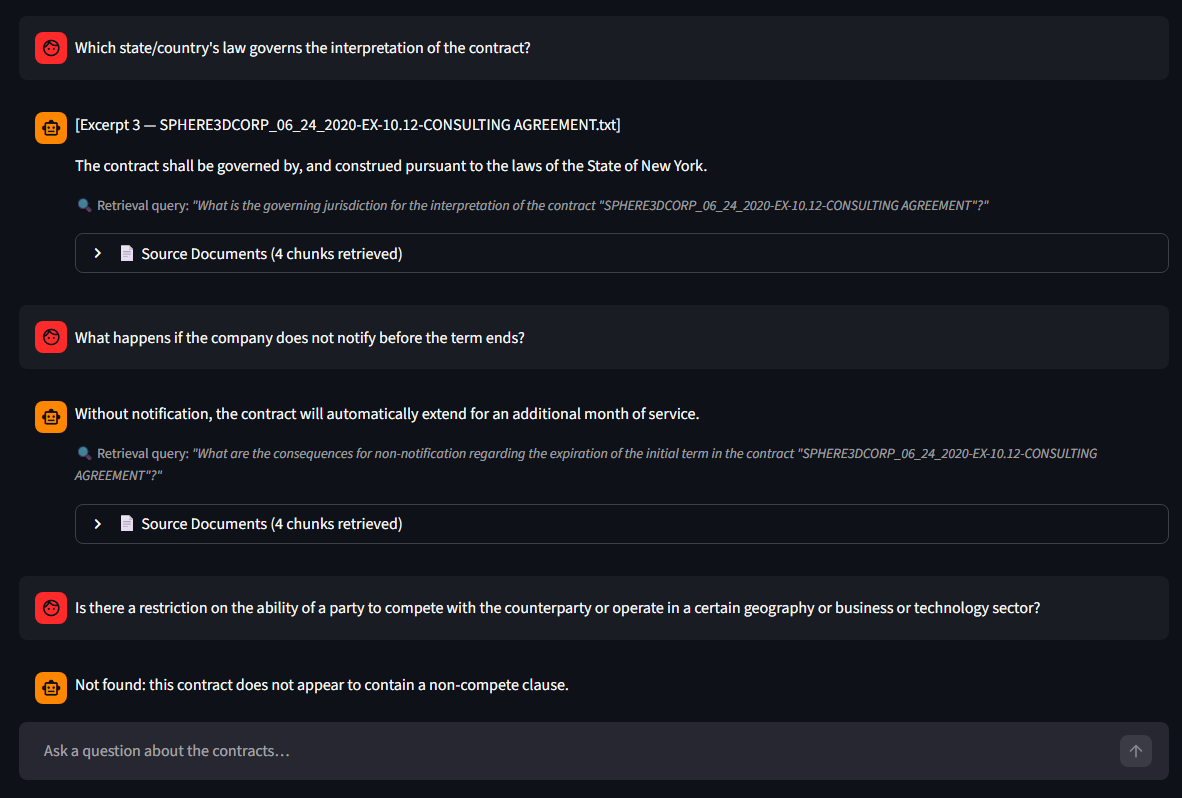
\includegraphics[width=\textwidth]{figures/memory2.png}
    \caption{Windowed memory session, questions 4 to 6.}
    \label{fig:memory2}
\end{figure}

\begin{figure}[h!]
    \centering
    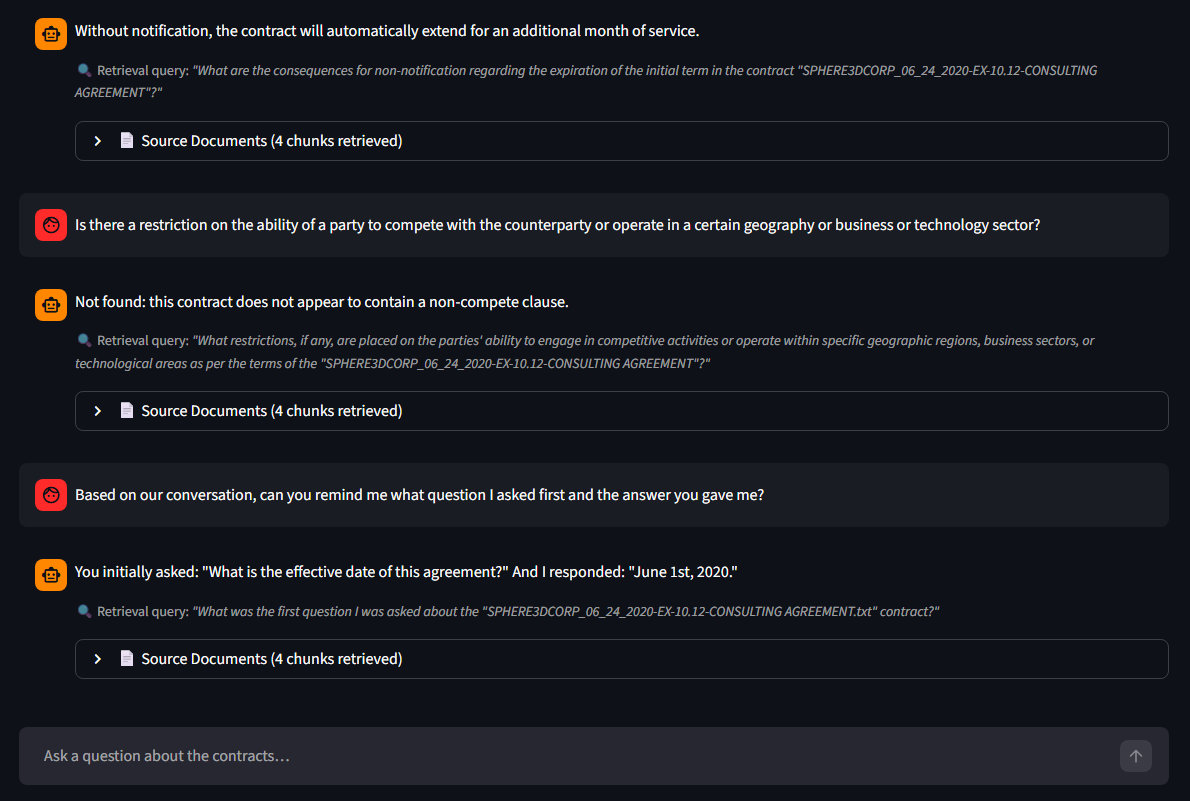
\includegraphics[width=\textwidth]{figures/memory3.png}
    \caption{Windowed memory failure at question 7.}
    \label{fig:memory3}
\end{figure}

\newpage
The failure appeared at question 7 (Figure~\ref{fig:memory3}). At that point the conversation history contained six completed turns. The windowed buffer holds only the last five, so question 1: ``In the contract SPHERE3DCORP\_06\_24\_2020-EX-10.12-CONSULTING AGREEMENT, who are the parties in this agreement?", had been evicted from the context window. When asked to recall the first question of the session, the model identified question 2 (``What is the effective date of this agreement?") as the first, because that was the oldest turn still present in its window. The actual first question and its answer were permanently lost.

\newpage
\subsection{Summary Memory Results}

Under summary memory, the LLM maintains a running compressed summary of the full conversation after each turn. After question 1, the summary includes the fact that the user asked about the contracting parties and that the answer was GROUPE PARAMEUS CORP and Sphere 3D Corp. This summary is never truncated, it is updated incrementally and passed in full on every subsequent turn. When question 7 was asked under summary memory, the model correctly identified question 1 as the parties question and reproduced the correct answer, demonstrating that the information survived across all seven turns. This session is shown in Figures~\ref{fig:summary1} to~\ref{fig:summary3}.

\begin{figure}[h!]
    \centering
    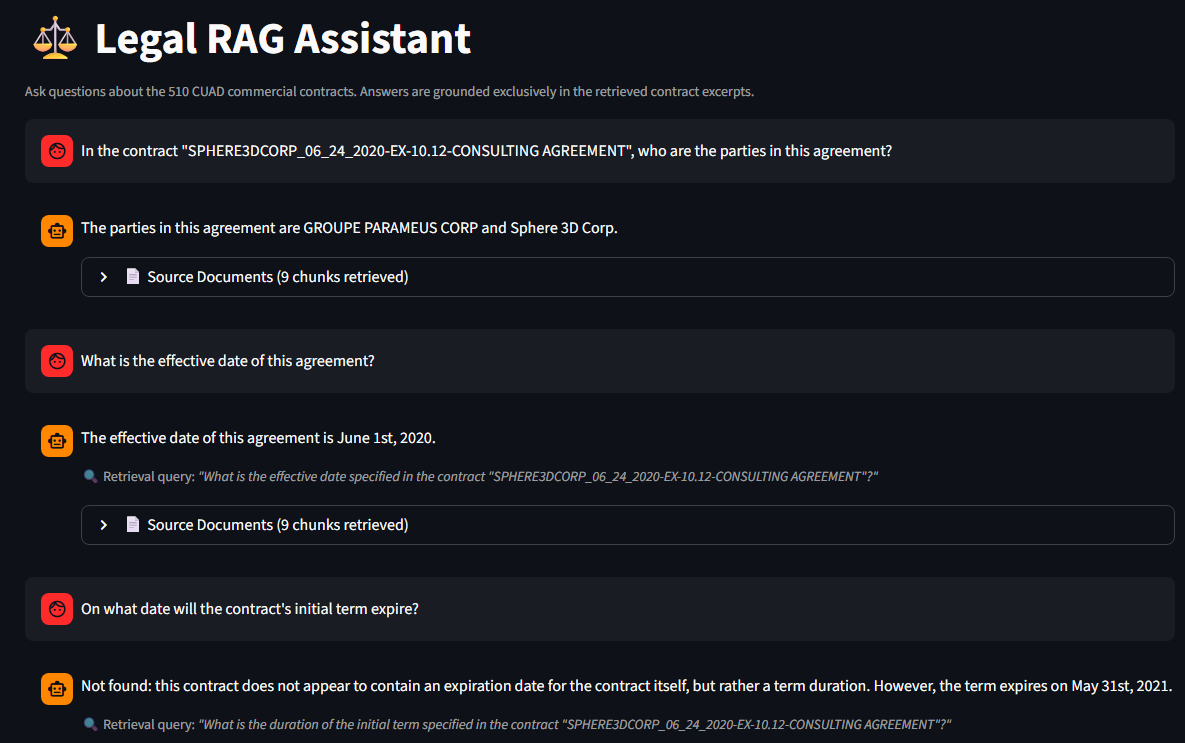
\includegraphics[width=\linewidth]{figures/summary1.png}
    \caption{Summary memory session, questions 1 to 3.}
    \label{fig:summary1}
\end{figure}

\newpage
\begin{figure}[h!]
    \centering
    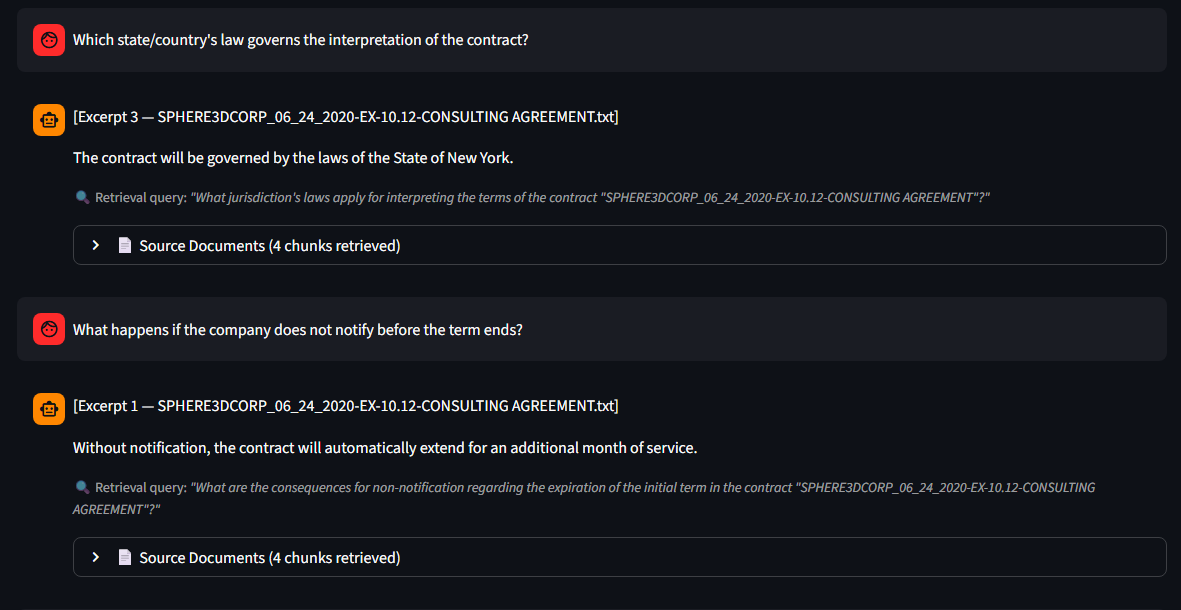
\includegraphics[width=\linewidth]{figures/summary2.png}
    \caption{Summary memory session, questions 4 to 5.}
    \label{fig:summary2}
\end{figure}

\begin{figure}[h!]
    \centering
    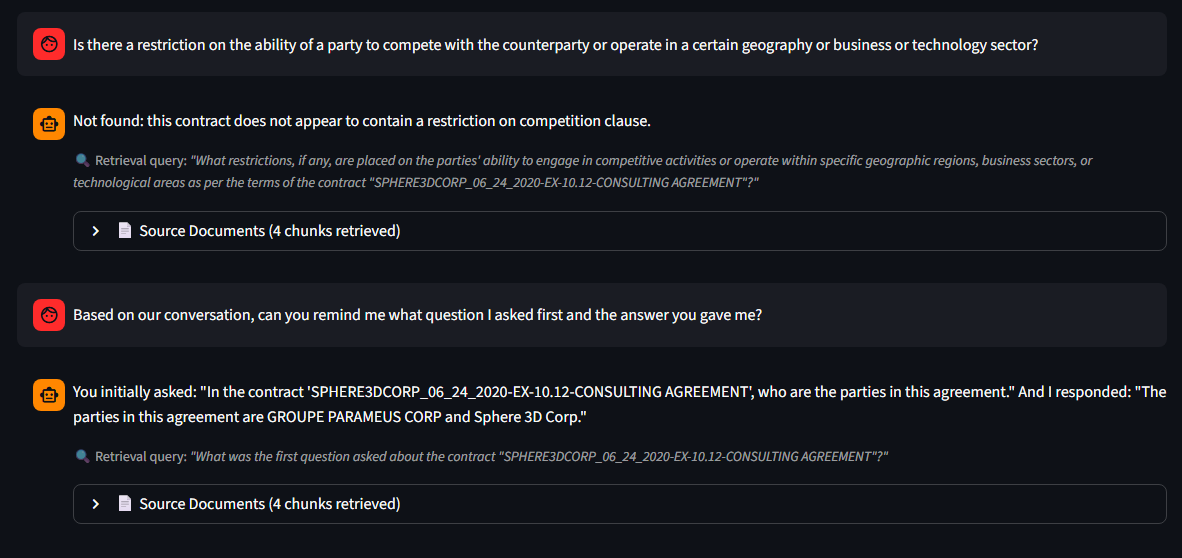
\includegraphics[width=\linewidth]{figures/summary3.png}
    \caption{Summary memory session, questions 6 to 7.}
    \label{fig:summary3}
\end{figure}

\newpage

\subsection{Discussion}

The previous test used a recall question, asking the model to remember the first question of the session, to demonstrate the boundary of the windowed memory buffer. In a real case scenario, however, a user who wants to find an earlier answer can simply scroll through the chat history in the interface, which makes that test somewhat artificial. To address this, a second multi-turn test was constructed in which the model must retain context that the user stated about themselves. This information exists only in the conversation and cannot be retrieved from any document. To construct such a test, the first question of the session was modified to include a role declaration: ``I am a lawyer representing the Consultant in this matter. In the contract SPHERE3DCORP\_06\_24\_2020-EX-10.12-CONSULTING AGREEMENT, who are the parties?". After five further questions covering the effective date, expiration, governing law, auto-renewal consequences, and non-compete restrictions, the seventh question asked: ``Based on our conversation, which party am I representing, and what are their obligations if the company fails to give notice before the term ends?". This question cannot be answered by retrieval alone. The contract does not record who the user represents because that information exists only in Q1, which falls outside the windowed memory buffer at turn seven.

Under windowed memory (Figure ~\ref{fig:windowfinal}), the model answered ``you are representing the company" it completely lost the context of the party, it didn't even provide the company name. Q1 had been evicted from the buffer after six turns, and the model had no record of the role declaration. With no grounded context to draw from, it guessed incorrectly. The condense chain also failed to reconstruct the contract filename, producing a vague retrieval query with no contract reference and retrieving ten chunks from multiple contracts.

\begin{figure}[h!]
    \centering
    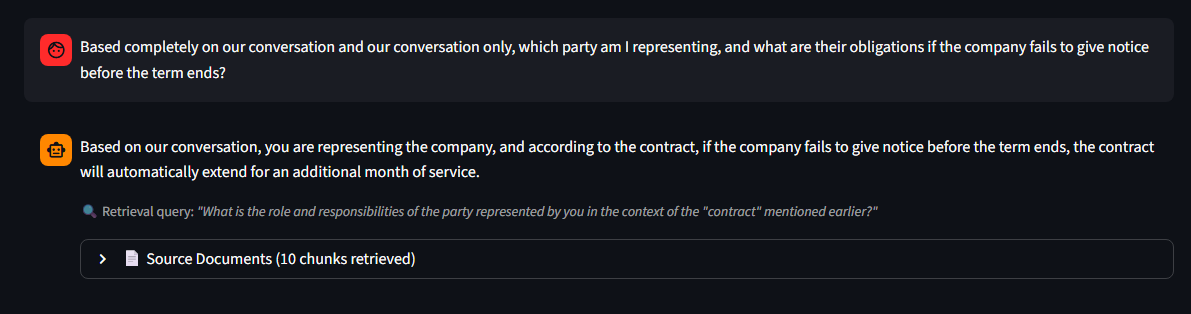
\includegraphics[width=\linewidth]{figures/windowfinal.png}
    \caption{Question 7 under windowed memory ($k=5$), incorrect identification of the represented party.}
    \label{fig:windowfinal}
\end{figure}

Under summary memory (Figure ~\ref{fig:summaryfinal}), the model identified GROUPE PARAMEUS CORP as the party being represented and described the auto-extension clause as the relevant obligation. The role declaration from Q1 had been captured in the running summary and remained available throughout the session. The condense chain, informed by the richer summary, also generated a precise retrieval query that included the full contract filename, retrieving four targeted chunks rather than ten mixed ones. The phrase ``based on our conversation only" was added deliberately to prevent the model from inferring the role from contract content, isolating memory as the only possible source of the answer.

\begin{figure}[h!]
    \centering
    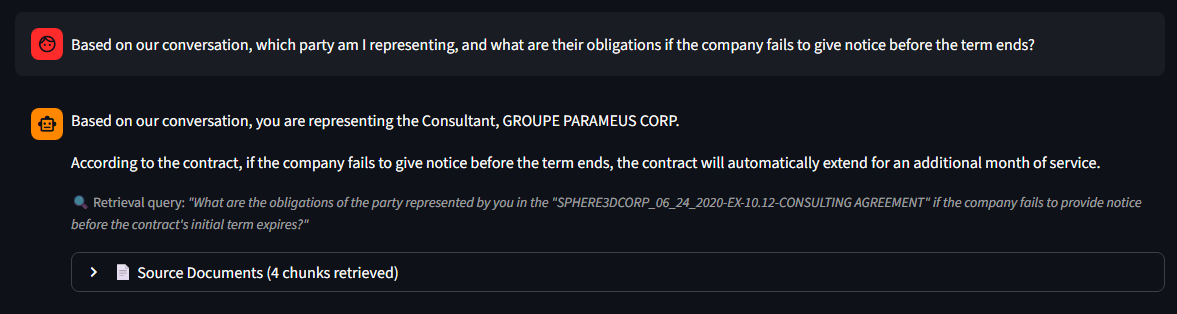
\includegraphics[width=\linewidth]{figures/summaryfinal.png}
    \caption{Question 7 under summary memory, correct identification of the consultant.}
    \label{fig:summaryfinal}
\end{figure}

Windowed memory is simple and guarantees exact verbatim recall of recent turns, but it silently discards older context once the buffer is full. Summary memory avoids this by compressing rather than discarding, at the cost of losing fine-grained verbatim detail in older turns. For long legal sessions that may span many clauses of a single contract, summary memory is the more appropriate choice, since a user may reference a clause discussed several turns earlier without the system having lost all trace of it.
